% This is figure 1. It contains model and results validating the model.
\RequirePackage{luatex85,shellesc}
\documentclass[varwidth=11.4cm,multi=false,crop,class=../pnas-new]{standalone}
\usepackage{pgfplots}
\pgfplotsset{compat=newest}
\usepackage[T1]{fontenc}
% \usepackage[sfdefault]{FiraSans}
\usepackage[small,euler-digits]{eulervm}
\renewcommand\familydefault{\sfdefault}

\usepackage{siunitx}
\usetikzlibrary{positioning,calc}
\usepgfplotslibrary{units}

\begin{document}

\edef\figW{11.4}
\edef\plotH{3}
\pgfmathsetmacro{\colW}{0.5*\figW}
\pgfmathsetmacro{\plotW}{0.9*\colW}
\pgfmathsetmacro{\VGapBetweenAxis}{-15mm}
\renewcommand\familydefault{\sfdefault}
\newcommand\LABELAXIS[2]{\node[above left=of #1.north west,yshift=-9mm] (#1.label) {\bf #2};}

\pgfplotsset{
    , xtick align=center
    , ytick align=center
    , unit markings=parenthesis
    , legend style={fill=none,draw=none,font=\footnotesize}
    , axis lines=left
    , axis line style={-}
    , title style={yshift=-2mm}
    , label style={font=\small}
    , tick label style={font=\scriptsize}
}

\pgfmathsetmacro{\plotAW}{0.35*\figW}
\pgfmathsetmacro{\plotBW}{0.55*\figW}

\begin{tikzpicture}[scale=1, every node/.style={} ]
    \node[label=north west:{\bf A} ] (model)
    {
        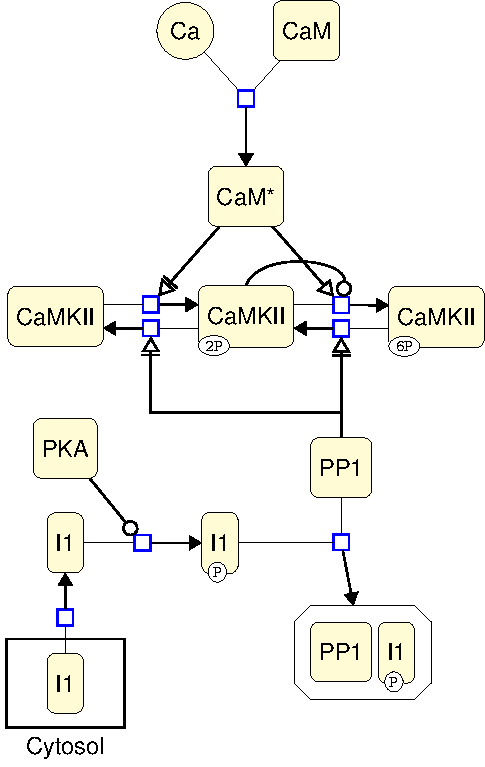
\includegraphics[width=\plotAW cm]{./model_sbgn_pd.pdf} 
    };

    \node[below=of model.south west, anchor=north west, label=north west:{\bf B}] (reac) 
    {
        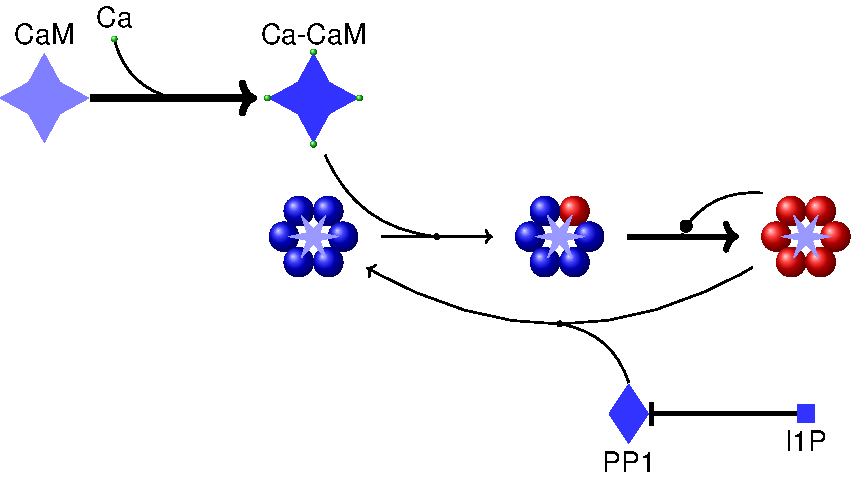
\includegraphics[width=\plotAW cm]{./camkii_pp1_switch_level1_detail.pdf} 
    };
    \node[below=of reac,yshift=1cm] (su) {
        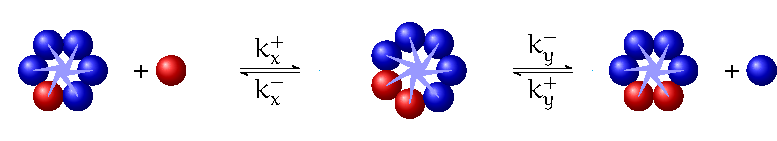
\includegraphics[width=\plotAW cm]{./camkii_subunit_exchage.pdf}
    };

    // Side figure.
    \begin{axis}[ name=C
        , at={(model.north east)}, anchor=north west
        , xshift=15mm
        , xlabel=Time, x unit=sec
        , title={Ca input}
        , y unit=\si{\nano M}
        , width=\plotBW cm, height=\plotH cm
        , enlarge y limits
        , enlarge x limits={abs=1}
    ]
        \addplot [blue, thick] gnuplot [ raw gnuplot ] {
            mod(x,y)=x-floor(x/y)*y;
            b=80;
            f(t)=(mod(floor(t),4)>=2)?b:b*(1+rand(0));
            plot [t=0:20] f(t);
        };
    \end{axis} 
    \LABELAXIS{C}{C}

    % \node[xshift=-1.5cm,yshift=5mm] at (C.north west) {\bf C};
    \begin{axis}[ name=D
        , at=(C.south west), anchor=north west, yshift=-15mm
        , width=\plotBW cm, height=\plotH cm
        , xtick={0,0.5,1.0,1.5,2.0}
        , enlarge y limits
        , ylabel={Active Fraction}
        , title={N\textsubscript{CaMKII}=15}
        % , title style={at={(0.15,1)}}
        , xlabel=Time, x unit=day
        ]
        \addplot [color=blue] gnuplot [ raw gnuplot ] {
            plot "./_data/camkii_15_200_days.dat" every 5::::10000
            using (column("time")/86400/30):(column("CaMKII*")/15)
        };
    \end{axis}
    \LABELAXIS{D}{D}
    \begin{axis}[ name=D2, at=(D.south west), anchor=north west, yshift=\VGapBetweenAxis
            , xlabel=Time, x unit=month
            , width=\plotBW cm, height=\plotH cm
            % , xmin = 0, xmax = 120
            , xtick={20,40,60,80,100,120}
            , enlarge y limits
            , ylabel={Active Fraction}
            , title={N\textsubscript{CaMKII}=35}
            % , title style={at={(0.15,1)}}
        ]
        \addplot [color=blue] gnuplot [ raw gnuplot ] {
            plot "./_data/camkii_35_long.dat" every 100 
            using (column("time")/86400/30):(column("CaMKII*")/35)
        };
    \end{axis}
    \begin{semilogyaxis}[ name=E
        , at=(D2.south west), anchor=north west
        , yshift = \VGapBetweenAxis
        , xlabel = N\textsubscript{CaMKII}
        , width = 0.75*\plotBW cm
        , ylabel = Kramer Time, y unit=day
        , legend style={font=\scriptsize,fill=white,at={(0.65,0.1)},anchor=south west}
        , enlargelimits, grid
        ]
        \addplot[only marks, blue, thick, mark size=2pt,mark=o] table 
            [col sep=comma,x=CaMKII,y=CramerTime] {./_data/switch_stability.csv};
        \addplot [domain=5:40, blue, very thick, smooth, solid, no markers] {exp((x-8)/4.2)};
        \legend{Simulation data,fit $\exp{\left(\frac{N_\text{CaMKII}-8}{4.2}\right)}$}
    \end{semilogyaxis}
    \LABELAXIS{E}{E}
\end{tikzpicture}
\end{document}
